\chapter{Diagonalization for Poisson}

\section{Direct method based on diagonalization}

Let us now consider a different way of solving the finite difference equations
we derived in the context of discretizing the Poisson problem. The method is
based on \emph{diagonalization}, and we first explain the approach in the context
of the one-dimensional Poisson problem:

\begin{align*}
  -u_{xx} &= f \quad \text{in}\, \Omega = (0,1), \\
  u(0) = u(1) &= 0.
\end{align*}
Assume that we use a uniform finite difference grid given by:
\begin{equation*}
  x_i = x_0 + ih, \quad i=0,1,\ldots,n.
\end{equation*}

The corresponding system of algebraic equations can be written as
\begin{align*}
  \frac{1}{h^2}
  \begin{pmatrix}
    2 & -1 & & & \\
    -1 & 2 & -1 & & \\
    & -1 & 2 & -1 & \\
    & & & \ddots & -1 \\
    & & & -1 & 2
  \end{pmatrix}
  \begin{pmatrix}
    u_1 \\
    u_2 \\
    \vdots \\
    u_{n-1}
  \end{pmatrix}
  =
  \begin{pmatrix}
    f_1 \\
    f_2 \\
    \vdots \\
    f_{n-1}
  \end{pmatrix},
\end{align*}
where $u_i$ is an approximation to $u(x_i) = u(ih),$ $i=1,\ldots,n-1$,
$f_i=f(x_i)$, and $u_0 = u_n = 0$ due to the specified boundary conditions. Let us write this system as

\begin{align*}
  \frac{1}{h^2} \matT \uu = \bff
\end{align*}
where
\begin{align*}
  \matT =
  \begin{pmatrix}
    2 & -1 & & & \\
    -1 & 2 & -1 & & \\
    & -1 & 2 & -1 & \\
    & & & \ddots & -1 \\
    & & & -1 & 2
  \end{pmatrix} , \qquad
  \uu =
  \begin{pmatrix}
    u_1 \\
    \vdots \\
    u_{n-1}
  \end{pmatrix} , \qquad
  \bff =
  \begin{pmatrix}
    f_1 \\
    \vdots \\
    f_{n-1}
  \end{pmatrix},
\end{align*}
and $h$ is the grid size or mesh size. Since $\matT$ is symmetric
positive definite, it can be \emph{diagonalized}.

\subsection{Diagonalization of $\matT$}

Diagonalization of $\matT$ means that we wish to find the eigenvalues
$\lambda_j$ and the eigenvectors $\matQ_j$ of $\matT$,
\begin{align*}
  \matT \matQ_j &= \lambda_j \matQ_j \quad j=1,\ldots,n-1,
\end{align*}
where
\begin{align*}
  \lambda_j &> 0 \qquad &\text{(positive eigenvalues)}, \\
  \matQ_k^\intercal \matQ_j &= \delta_{jk} \qquad &\text{(orthonormal eigenvectors)}.
\end{align*}

We collect all the eigenvectors $\matQ_j$ into the orthogonal matrix $\matQ$,
\begin{equation*}
  \matQ = \begin{pmatrix} \matQ_1 & \matQ_2 & \cdots & \matQ_{n-1}\end{pmatrix}.
\end{equation*}
Then
\begin{align*}
  \matT \matQ &= \matQ \bm \Lambda
\end{align*}
where
\begin{align*}
  \bm \Lambda &= \operatorname{diag}(\lambda_1, \ldots, \lambda_{n-1}) =
  \begin{pmatrix}
    \lambda_1 & & \\
     & \ddots & \\
    & & \lambda_{n-1}
  \end{pmatrix}.
\end{align*}
Since
\begin{align*}
  \matQ^\intercal \matQ = \bm I =
  \begin{pmatrix}
    1 & & \\
    & \ddots & \\
    & & 1
  \end{pmatrix} \qquad
  \Rightarrow \quad \matQ^\intercal = \matQ^{-1},
\end{align*}
and
\begin{align}
  \matT &= \matQ \bm \Lambda \matQ^\intercal
  \label{eq:T_diag}
\end{align}
or
\begin{align*}
  \matQ^\intercal \matT \matQ = \bm \Lambda \qquad \text{(diagonal)}.
\end{align*}

Following this approach the finite difference approximation can be computed as
follows:
\begin{alignat*}{2}
  \bm g &\equiv  h^2 \bff \quad &  \qquad \qquad \bm g
  &: \; \mathcal{O}(n) ~ \text{operations} \\
  \\
  \matT \, \uu &= \bm g \\
  \matQ \, \bm \Lambda \, \matQ^\intercal \uu &= \bm g \\
  \bm \Lambda \underbrace{\matQ^\intercal \uu}_{\tilde{\uu}}
  &= \underbrace{\matQ^\intercal \bm g}_{\tilde{\bm g}}
  & \tilde{\bm g} &: \; \mathcal{O}(n^2) ~ \text{operations} \\
  \\
  \bm \Lambda \tilde{\uu} &= \tilde{\bm g} \\
  \tilde{\uu} &= \bm \Lambda^{-1} \tilde{\bm g}
  & \tilde{\uu} &: \; \mathcal{O}(n) ~ \text{operations} \\
  \\
  \matQ^\intercal \uu &= \tilde{\uu} \\
  \uu &= \matQ \tilde{\uu} & \uu
  &: \; \mathcal{O}(n^2) ~ \text{operations}
\end{alignat*}
Note that the transformations
\begin{equation*}
  \tilde{\bm g} = \matQ^\intercal \bm g \quad \text{and} \quad \uu = \matQ \tilde{\uu}
\end{equation*}
are \emph{matrix-vector products}. In summary, we can compute $\uu$ in
\begin{equation*}
  \mathcal{O}(n) + \mathcal{O}(n^2) + \mathcal{O}(n) + \mathcal{O}(n^2)
  \sim \mathcal{O}(n^2) ~ \text{floating-point operations}.
\end{equation*}
Hence, we can solve our finite difference system in $(n-1)$ unknowns in
$\mathcal{O}(n^2)$ operations. This is \emph{not} competitive with a direct
solution algorithm based upon LU-factorization (Gaussian elimination) of a
tridiagonal matrix, which can be done in $\mathcal{O}(n)$ operations (since the
bandwidth is equal to one).

Let us also compare the memory requirement:
\begin{align*}
  &\mathcal{O}(n^2) ~\text{for the diagonalization approach
  (we need to store $\matQ$)}; \\
  &\mathcal{O}(n) ~\text{for a tridiagonal direct solver}.
\end{align*}
Again, the diagonalization approach is {\em not} competitive.

So, why bother? The answer is that the diagonalization approach becomes more
interesting in $\mathbb{R}^2$. In addition, we will later see how we can use the
Fast Fourier Transform (FFT) to lower the computational complexity.

\section{The Poisson problem in $\mathbb{R}^2$}

The two-dimensional Poisson problem on the unit square is given by

\begin{equation}
  \begin{split}
    -\nabla^2 u &= f \qquad \text{in} ~ \Omega=(0,1) \times (0,1), \\
    u &= 0 \qquad \text{on} ~ \partial \Omega, \\
  \end{split}
  \label{eq:Poisson2D}
\end{equation}
where
\[
  \nabla^2 u = \frac{\partial^2 u}{\partial x^2}
  + \frac{\partial^2 u}{\partial y^2}.
\]

%XXX
%\begin{figure}
%  \centering
%  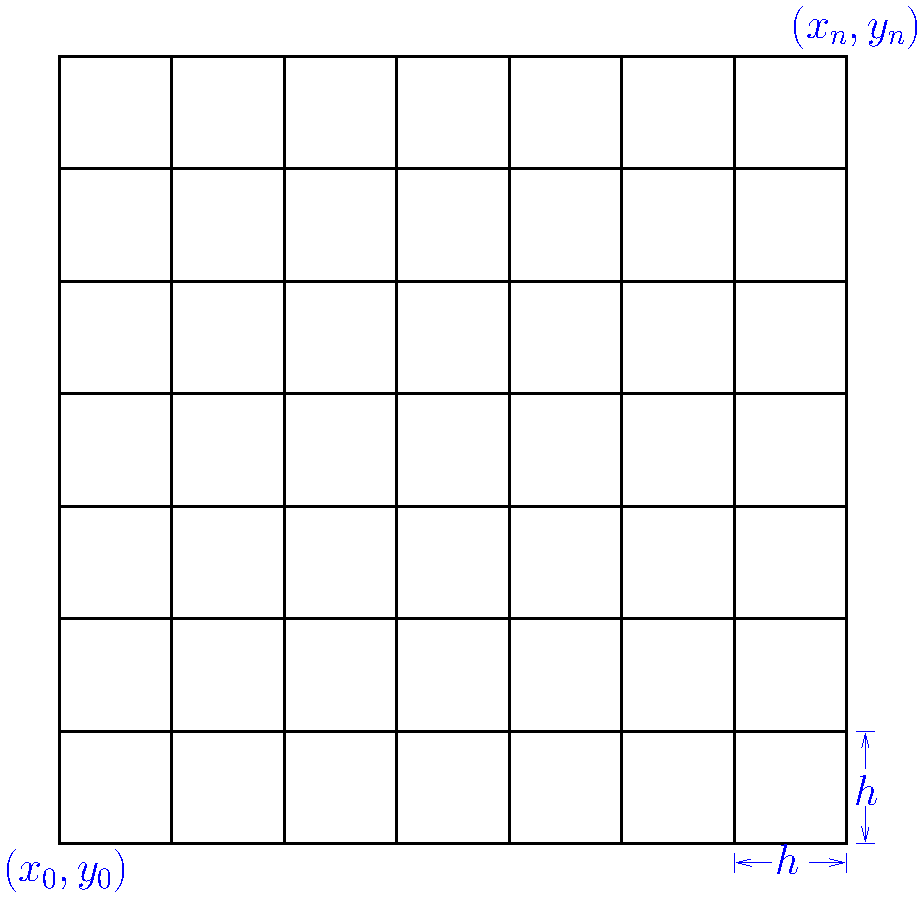
\includegraphics[width=8cm]{FiniteDifferenceGrid}
%    \caption{A uniform finite difference grid.}
%  \label{fig:FDM_grid_2D}
%\end{figure}

Again, using the notation $u_{i,j} \simeq u(x_i,y_j) = u(i h, j h)$ and
$f_{i,j}=f(x_i,y_j)$, and discretizing \eqref{eq:Poisson2D} using the 5-point
stencil (see Figure \ref{fig:FDM_grid_2D}), the discrete equations read
\begin{equation}
  -\frac{(u_{i+1,j}-2u_{i,j}+u_{i-1,j})}{h^2} - \frac{(u_{i,j+1}-2u_{i,j}+u_{i,j-1})}{h^2} = f_{i,j}
  \label{eq:FDM_sys}
\end{equation}
for $1 \leq i,j \leq n-1$.

\subsection{Diagonalization}

Let
\begin{equation*}
  \uu =
  \begin{pmatrix}
    u_{1,1} & \cdots & u_{1,n-1} \\
    \vdots & \ddots & \vdots \\
    u_{n-1,1} & \cdots & u_{n-1,n-1}
  \end{pmatrix}
\end{equation*}
and
\begin{equation*}
  \matT =
  \begin{pmatrix}
    2 & -1 & & & \\
    -1 & 2 & -1 & & \\
    & & \ddots & & \\
    & & -1 & 2 & -1 \\
    & & & -1 & 2
  \end{pmatrix}.
\end{equation*}

Then,
\begin{alignat*}{2}
  (\matT \uu)_{ij} &= 2u_{i,j} - u_{i+1,j}, & \qquad i=1, \\
  (\matT \uu)_{ij} &= -u_{i-1,j}+2u_{i,j} - u_{i+1,j}, &\qquad 2 \leq i \leq n-2, \\
  (\matT \uu)_{ij} &= -u_{i-1,j}+2u_{i,j}, &\qquad i=n-1.
\end{alignat*}
and thus,
\begin{equation}
  \frac{1}{h^2} (\matT \uu)_{ij} \simeq
  - \left( \frac{\partial^2 u}{\partial x^2} \right)_{i,j}.
\end{equation}

Similarly in the other direction,
\begin{equation}
  \frac{1}{h^2} (\uu \matT)_{ij} \simeq
  - \left( \frac{\partial^2 u}{\partial y^2} \right)_{i,j}.
\end{equation}

Our finite difference system (\ref{eq:FDM_sys}) can thus be expressed as
\begin{equation*}
  \frac{1}{h^2} (\matT \uu + \uu \matT)_{ij} = f_{i,j}
  \qquad \text{for} \qquad 1 \leq i,j \leq n-1, \\
\end{equation*}
or
\begin{equation}
  \matT \uu + \uu \matT = \bm G
  \label{eq:Poisson2D_TUUT}
\end{equation}
where
\begin{equation*}
  \bm G = h^2
  \begin{pmatrix}
    f_{1,1} & \ldots & f_{1,n-1} \\
    \vdots & \ddots & \vdots \\
    f_{n-1,1} & \ldots & f_{n-1,n-1}
  \end{pmatrix}.
\end{equation*}

Combining \eqref{eq:T_diag} and \eqref{eq:Poisson2D_TUUT} we get
\begin{equation}
  \matQ \bm \Lambda \matQ^\intercal \uu + \uu \matQ \bm \Lambda \matQ^\intercal = \bm {G}.
  \label{eq:Poisson2D_T_diag}
\end{equation}

Multiplying \eqref{eq:Poisson2D_T_diag} from the right with $\matQ$ and from the
left with $\matQ^\intercal$, and using the fact that $\matQ^\intercal \matQ =
\bm I$, we get
\begin{equation*}
  \bm \Lambda \underbrace{\matQ^\intercal \uu \matQ}_{\tilde{\uu}} +
  \underbrace{\matQ^\intercal \uu \matQ}_{\tilde{\uu}} \bm \Lambda =
  \underbrace{\matQ^\intercal \bm G \matQ}_{\tilde{\bm G}}.
\end{equation*}

Hence, (\ref{eq:Poisson2D_TUUT}) may be solved in three steps:

\begin{enumerate}
\item Compute $\tilde{\bm G}$ using matrix-matrix products
  \begin{equation*}
    \tilde{\bm G} = \matQ^\intercal \bm G \matQ.
  \end{equation*}
\item Solve for $\tilde{\uu}$.
  \begin{align*}
    \bm \Lambda \tilde{\uu} + \tilde{\uu} \bm \Lambda &= \tilde{\bm G} \\
    \lambda_i \tilde{u}_{ij} + \tilde{u}_{ij} \lambda_j &= \tilde{g}_{ij} \\
    \tilde{u}_{ij} &= \frac{\tilde{g}_{ij}}{\lambda_i + \lambda_j}
  \end{align*}
\item Compute $\uu$ using matrix-matrix products
  \begin{equation*}
    \uu = \matQ \tilde{\uu} \matQ^\intercal
  \end{equation*}
\end{enumerate}

Here,
\begin{equation*}
  \uu, \tilde{\uu}, \tilde{\bm G}, \matQ \in \mathbb{R}^{(n-1) \times (n-1)}
\end{equation*}

\subsubsection{Computational cost}

The number of degrees of freedom (or unknowns) $N$ is
\begin{align*}
N = (n-1)^2 \sim \mathcal{O}(n^2) \quad (n \gg 1).\\
\end{align*}

\begin{enumerate}
\item Two matrix-matrix products give $\mathcal{O}(n^3)$ operations.
\item $\mathcal{O}(n^2)$ scalar constant time operations give $\mathcal{O}(n^2)$.
\item Two matrix-matrix products give $\mathcal{O}(n^3)$ operations.
\end{enumerate}
In summary, we can compute the discrete solution, $\uu$, in
$\mathcal{O}(n^3)=\mathcal{O}(N^{3/2})$ operations.

Note: this method is an example of a {\em direct method}.

\subsubsection{Comparison with other direct methods}

\begin{table}
    \caption{
      Computational cost and memory requirement for three different
      direct methods. The number of unknowns is $N=\mathcal{O}(n^2)$. For the
      banded solver, we have used a bandwidth $b \sim \mathcal{O}(n)$. Full LU
      means LU-factorization without exploiting sparsity.
    }
    \label{tab:DirectMethods_ComputationalCost}
  \begin{center}
    \bgroup\def\arraystretch{1.2}
    \begin{tabular}{lrr}
      \hline
      Method & Operations ($\mathcal{N}_\text{op}$) & Memory requirement ($\mathcal{M}$) \\
      \hline
      Diagonalization & $\mathcal{O}(N^{3/2}) = \mathcal{O}(n^3)$ & $\mathcal{O}(N) = \mathcal{O}(n^2)$ \\
      Banded LU & $\mathcal{O}(N b^2) = \mathcal{O}(n^4)$ & $\mathcal{O}(Nb) = \mathcal{O}(n^3)$ \\
      Full LU & $\mathcal{O}(N^3) = \mathcal{O}(n^6)$ & $\mathcal{O}(N^2) = \mathcal{O}(n^4)$ \\
      \hline
    \end{tabular}
    \egroup
  \end{center}
\end{table}

We conclude that the diagonalization method is much more attractive in
$\mathbb{R}^2$ than in $\mathbb{R}^1$. The number of floating-point operations
per degree of freedom is $\mathcal{O}(n)$, while the memory requirement is close to optimal (i.e. scalable).

\subsubsection{The matrices $\matQ$ and $\bm \Lambda$}

The computational cost associated with the diagonalization approach tacitly
assumes that we know the eigenvector matrix $\matQ$ and the corresponding
eigenvalues. Let us therefore derive explicit expressions for these. To this
end, consider first the continuous eigenvalue problem
\begin{equation*}
  \begin{split}
    -u_{xx} &= \lambda u \qquad \qquad \text{in } \Omega=(0,1), \\
    u(0) = u(1) &= 0,
  \end{split}
\end{equation*}
with solutions
\begin{equation*}
  \begin{split}
    \bar{u}_j(x) &= \sin(j \pi x), \\
    \bar{\lambda}_j &= j^2 \pi^2,
  \end{split}
  \qquad j=1,2,\ldots,\infty.
\end{equation*}

Consider now the discrete eigenvalue problem
\begin{equation*}
  \matT \tilde{\matQ}_j =
  \lambda_j \tilde{\matQ}_j
\end{equation*}
Try eigenvector solutions which correspond to the continuous eigenfunctions
$\bar{u}_j(x)$ sampled at the grid points $x_i, i=1,\ldots,n-1$, i.e.
\begin{equation*}
  \begin{split}
    (\tilde{\matQ}_j)_i &= \bar{u}_j (x_i) \\
    &= \sin(j \pi x_i) \\
    &= \sin(j \pi (i h)), \\
    &= \sin \left(\frac{i j \pi}{n} \right)
  \end{split}
\end{equation*}

Operating on $\tilde{\matQ}_j$ with $\matT$ gives
\begin{equation*}
  (\matT \tilde{\matQ}_j)_i =
  \underbrace{2\left( 1 - \cos\left( \frac{j\pi}{n} \right) \right)}_{\lambda_j}
  \underbrace{\sin\left( \frac{i j \pi}{n} \right)}_{(\tilde{\matQ}_j)_i}
\end{equation*}

Hence, our try was successful: operating on $\tilde{\matQ}_j$ with $\matT$ gives
a multiple of $\tilde{\matQ}_j$.

In order to proceed, set $\matQ_j = \alpha \tilde{\matQ}_j$, and choose $\alpha$
such that $\matQ_j$ is normalized:

\begin{align*}
  (\matQ_j)_i &= \sqrt{\frac{2}{n}} \sin \left( \frac{ij \pi}{n} \right),
                \qquad \qquad 1 \leq i,j \leq n-1, \\
  \lambda_j &= 2 \left( 1 - \cos \left( \frac{j \pi}{n} \right) \right).
\end{align*}

For ${j \ll n}$, we observe that
\begin{align*}
  \lambda_j
  &\simeq 2 \left( 1 - \left( 1 -\frac{1}{2} \frac{j^2 \pi^2}{n^2} + \ldots \right) \right)
    \simeq \frac{j^2 \pi^2}{n^2}. \\
  \intertext{Since $h=1/n$, we have}
  \lambda_j &\simeq h^2j^2 \pi^2 = h^2 \bar{\lambda}_j \qquad \text{ for } j \ll n.
\end{align*}

Since the approximation of the one-dimensional Laplace operator on our finite
difference grid is equal to $\matT / h^2$, this is the same as saying that the
first, lowest eigenvalues (and eigenvectors) for the continuous case are well
approximated by our finite difference formulation.

Note that
\begin{align*}
 \matQ_{ij}
  &= (\matQ_j)_i = \sqrt{\frac{2}{n}} \sin \left( \frac{ij \pi}{n} \right),
    \qquad 1 \leq i,j \leq n-1, \\
\end{align*}
and that indeed
\begin{align*}
  \matQ^\intercal = \matQ, \qquad \matQ^\intercal \matQ = \bm I.
\end{align*}

From the comparison of the computational cost shown earlier, the diagonalization
approach to solving the discrete Poisson problem appears promising.

\textbf{Questions}:
\begin{enumerate}
\item Can the matrix-matrix multiplications be done fast?
\item Can the matrix-matrix multiplications be parallelized?
\item Can we do better?
\end{enumerate}

\subsubsection{Numerical results}

A diagonalization solver based on ``standard'' matrix-matrix product code (i.e.
no special library was used). The code was run on a PC, Pentium III with 512 MB
RAM (2000) and on a single processor on Gridur, MIPS R14000 with 1 GM RAM
(2006).

We define $\tau(n)$ as the total simulation time (in seconds), $\tau_1(n) =
\tau(n)/n^2$ as the time spent per degree of freedom, and
\[
  r(n) = \frac{\tau_1(n)}{\tau_1(n/2)}
\]
as the slowdown factor when doubling the problem size.

See \autoref{tbl:numres-diag}. The source code follows.

\begin{table}
  \caption{
    Simulation results for the numerical approximation of the two-dimensional
    Poisson equation by finite differences. The solution of the system of
    discrete equations is based on diagonalization techniques and matrix-matrix
    products. A listing of the FORTRAN program used in these tests is given
    below. It is interesting to note that the elapsed time on a single processor
    on Gridur is reduced by a factor of more than 80 compared to using the PC
    from 2000 when $n=1024$.
  }
  \label{tbl:numres-diag}
  \begin{center}
    \bgroup\def\arraystretch{1.2}
    \begin{tabular}{r|lll|ll}
      \hline
      \multicolumn{1}{r}{}
      & \multicolumn{3}{|c|}{PC (2000)}
      & \multicolumn{2}{c}{Gridur (2006)} \\
      \hline
      $n$ & $\tau(n)$ & $\tau_1(n)$ & $r(n)$ & $\tau(n)$ & $\tau_1(n)$ \\
      \hhline{======}
      $32$ & $1.80 \cdot 10^{-2}$ & $1.76 \cdot 10^{-5}$ & & &\\
      $64$ & $1.50 \cdot 10^{-1}$ & $3.66 \cdot 10^{-5}$ & $2.1$ & & \\
      $128$ & $1.20$ & $7.34 \cdot 10^{-5}$ & $2.0$ & $2.45 \cdot 10^{-2}$ & $1.50 \cdot 10^{-6}$ \\
      $256$ & $9.84$ & $1.50 \cdot 10^{-4}$ & $2.0$ & $0.167$ & $2.55 \cdot 10^{-6}$ \\
      $512$ & $103.9$ & $3.96 \cdot 10^{-4}$ & $2.6$ & $1.33$ & $5.08 \cdot 10^{-6}$ \\
      $1024$ & $873.2$ & $8.33 \cdot 10^{-4}$ & $2.1$ & $10.33$ & $9.85 \cdot 10^{-6}$ \\
      \hline
      & $\sim \mathcal{O}(n^3)$ & $\sim \mathcal{O}(n)$ & & & \\
      \hline
    \end{tabular}
    \egroup
  \end{center}
\end{table}

\begin{lstlisting}[style=fortran]
  program poisson

  ! Program to solve the two-dimensional Poisson equation on
  ! a unit square using one-dimensional eigenvalue decompositions
  ! and matrix-vector products.
  ! In this example, the right hand side f=1.

  ! Einar M. Ronquist
  ! NTNU, October 2000

  parameter (n = 256)
  parameter (m = n-1)

  real*8 diag(m), q(m,m), qt(m,m), b(m,m), u(m,m), w(m,m), pi
  real*4 tarray(2), t1, t2, dt

  t1 = etime(tarray)

  h  = 1./n
  pi = 4.*atan(1.)

  do i=1,m
    diag(i) = 2*(1-cos(i*pi/n))
  enddo

  do j=1,m
    do i=1,m
      q(i,j) = sin(i*j*pi/n) * sqrt((2./n))
    enddo
  enddo

  do j=1,m
    do i=1,m
      qt(i,j) = q(j,i)
    enddo
  enddo

  do j=1,m
    do i=1,m
      b(i,j) = h*h
    enddo
  enddo

  call mxm(b,m,q,m,w,m)
  call mxm(qt,m,w,m,b,m)

  do j=1,m
    do i=1,m
      u(i,j) = b(i,j)/(diag(i)+diag(j))
    enddo
  enddo

  call mxm(u,m,qt,m,w,m)
  call mxm(q,m,w,m,u,m)

  t2 = etime(tarray)
  dt = t2-t1
  write(6,*) ' '
  write(6,*) 'dt (total)= ',dt
  dt = dt/(n*n)
  write(6,*) 'dt (per dof)= ',dt

  stop
  end

  subroutine mxm (a,n1,b,n2,c,n3)

  ! matrix-matrix product c = a*b

  real*8 a(n1,n2), b(n2,n3), c(n1,n3)
  do j=1,n3
    do i=1,n1
      c(i,j) = 0.0
      do k=1,n2
        c(i,j) = c(i,j) + a(i,k)*b(k,j)
      enddo
    enddo
  enddo

  return
  end
\end{lstlisting}

\subsection{Fast diagonalization methods}

The most expensive operation in the diagonalization method introduced in the
previous section is of the type
\begin{align*}
  \bm v^* &= \matQ \bm v = \matQ^\intercal \bm v, \\
  \intertext{where}
  Q_{ij} &= \sqrt{\frac{2}{n}} \sin \left( \frac{ij \pi}{n} \right) \qquad \qquad 1 \leq i,j \leq n-1.
\end{align*}

We will now consider ways to obtain $\bm v^*$ in $\mathcal{O}(n \log n)$
operations instead of $\mathcal{O}(n^2)$.

\subsubsection{Discrete Fourier Transform (DFT)}

Consider a periodic function $v(x)$ with period $2 \pi$. Consider sampling this
function at the equidistant points $x_j$, $j=0,1,\ldots,N$ with $x_j=j h$,
$\quad h=2 \pi / N$. Let $v_j = v(x_j) = v(j h)$, $j=0,1,\ldots,N$.
\begin{figure}[h]
  \centering
  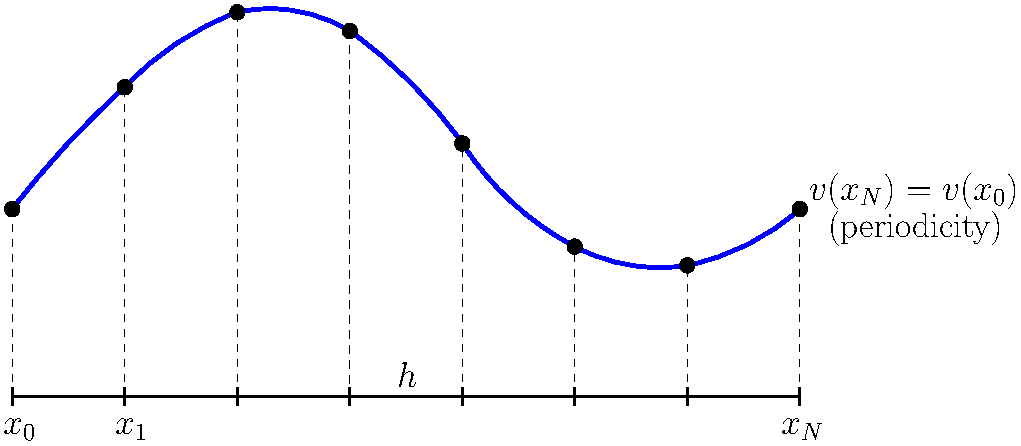
\includegraphics[width=10cm]{PeriodicFunction}
\end{figure}

Consider the vectors $\bm \varphi_k$, where
\begin{equation*}
  (\bm \varphi_k)_j = \text{e}^{\text{i} k x_j}, \qquad j,k=0,1,\ldots,N-1.
\end{equation*}

Note that the vector elements in $\bm \varphi_k$ represent the values of the
function $\varphi_k(x) = \text{e}^{\text{i}kx}$ sampled at the discrete points
$x_j, \quad j=0,1,\ldots,N-1$. Note also that the function $\varphi_k(x) =
\text{e}^{\text{i}kx}$ is an eigenfunction of the Laplace operator with periodic
boundary conditions.

The vectors $\{ \bm \varphi_k \}_{k=0}^{N-1}$ form a basis for the
$N$-dimensional vector space $\mathbb{C}^N$. In particular, we have that
\begin{equation*}
  \bm \varphi_k^\mathsf{H} \bm \varphi_l = N\delta_{kl},
  \qquad \qquad k,l=0,1,\ldots,N-1.
\end{equation*}

The vector
\begin{equation*}
  \bm v =
  \begin{pmatrix}
    v_0 & \cdots & v_{N-1}
  \end{pmatrix}^\intercal
  \in \mathbb{R}^N
\end{equation*}
can be expressed in this basis as
\begin{equation*}
  \bm v = \sum_{k=0}^{N-1} \hat{v}_k \bm \varphi_k \qquad \Rightarrow \qquad
  v_j = \sum_{k=0}^{N-1} \hat{v}_k (\bm \varphi_k)_j
        = \sum_{k=0}^{N-1} \hat{v}_k \text{e}^{\text{i} k x_j},
\end{equation*}
where $\hat{v}_k$, are the discrete Fourier coefficients given by
\begin{equation*}
  \hat{v}_k = \frac{1}{N} \sum_{j=0}^{N-1} v_j \text{e}^{-\text{i}k x_j}, \qquad \qquad
  \begin{matrix}
    x_j = j h \\
    h = 2\pi / N
  \end{matrix}
  \qquad k=0,1,\ldots,N-1
\end{equation*}

\subsubsection{Discrete Sine Transform (DST)}

The Discrete Sine Transform is applicable to a function $v(x)$ which is
\emph{periodic} with period $2 \pi$ and \emph{odd}. Discretize the function on
an equidistant grid on $[0,\pi]$ with $h=\pi/n$. Set
\begin{equation*}
  v_j = v(x_j) = v(jh) = v \left(\frac{j \pi}{n} \right), \qquad \qquad j=0,1,\ldots,n.
\end{equation*}

Since $v$ is odd,
\begin{equation*}
  v(x_0) = v(x_n) = 0.
\end{equation*}

The discretized function is therefore represented by the $(n-1)$ real values
$v_1,\ldots,v_{n-1}$, i.e. by the vector
\begin{equation*}
  \bm v = \begin{pmatrix} v_1 & \vdots & v_{n-1} \end{pmatrix}^\intercal
  \in \mathbb{R}^{n-1}.
\end{equation*}

An orthogonal basis for $\mathbb{R}^{n-1}$ is given by the vectors
$\bm \psi_k$, $k=1,\ldots,n-1$, where
\begin{align*}
  (\bm \psi_k)_j &= \sin \left( \frac{k j \pi}{n} \right), \qquad j=1,\ldots,n-1,
\end{align*}
and with
\begin{align*}
  \bm \psi_k^\intercal \bm \psi_l &=
  \begin{cases}
    \frac{n}{2}, & k=l, \\
    0, & k \not= 0.
  \end{cases}
\end{align*}

In terms of this basis, we can write $\bm v$ as
\begin{align*}
  v_j
  &= \sum_{k=1}^{n-1} \tilde{v}_k \sin \left( \frac{k j \pi}{n} \right), &\qquad j&=1,\ldots,n-1,
\end{align*}
where
\begin{align*}{2}
  \tilde{v}_k
  &= \frac{2}{n} \sum_{j=1}^{n-1} v_j \sin \left( \frac{j k \pi}{n} \right), &\qquad  k&=1,\ldots,n-1.
\end{align*}

We can also write this as $\tilde{\bm v} = \bm S \bm v$ (DST) and $\bm v = \bm
S^{-1} \tilde{\bm v}$ (inverse DST). Note that $\bm S$ and $\bm S^{-1}$ are
related as
\begin{equation*}
  \bm S = \frac{2}{n} \bm S^{-1}
\end{equation*}

Also note that
\begin{align*}
  \matQ = \sqrt{\frac{2}{n}} \bm S^{-1} = \sqrt{\frac{n}{2}} \bm S.
\end{align*}

Now, consider the matrix $\bff^{(N)}$ where
\begin{equation*}
  \begin{split}
    F_{k,j}^{(N)} &= \text{e}^{-\text{i}jkh} \\
    &= \cos \left( \frac{j k 2 \pi}{N} \right) -
    i \sin \left( \frac{j k 2 \pi}{N} \right),
    \qquad 0 \leq j,k \leq N-1.
  \end{split}
\end{equation*}

Note that
\begin{equation*}
  F_{k,j}^{(2 n)} = \cos \left( \frac{j k \pi}{n} \right)
  - i \sin \left( \frac{j k \pi}{n} \right), \qquad 0 \leq j,k \leq 2n-1.
\end{equation*}

Now, consider
\begin{align*}
  \bm v &= \begin{pmatrix} v_1 & \cdots & v_{n-1} \end{pmatrix}^\intercal \in \mathbb{R}^{n-1}.
\end{align*}
Construct the extended vector as an ``odd'' extension
\begin{align*}
  \bm w &= \begin{pmatrix} 0 & v_1 & \cdots & v_{n-1} & 0 & -v_{n-1} & \cdots & -v_1 \end{pmatrix}^\intercal
  \in \mathbb{R}^{2n}.
\end{align*}

First, note that
\begin{equation*}
  (\bff^{(2n)} \bm w)_k
  = \sum_{j=0}^{2n-1} \text{e}^{\frac{-\text{i}jk \pi}{n}} w_j
  = 2n \hat{w}_k,
\end{equation*}
where $\hat{w}$, $\quad k=0,1,\ldots,2n-1$ are the discrete Fourier coefficients. Second,
\begin{align*}
  (\bff^{(2n)} \bm w)_k
  &= \sum_{j=0}^{2n-1} \left[
    \cos \left( \frac{j k \pi}{n} \right)
    - i \sin \left( \frac{jk \pi}{n} \right)
    \right] w_j \\
  &= \sum_{j=0}^{2n-1} w_j \cos \left( \frac{jk \pi}{n} \right)
    - i \sum_{j=0}^{2n-1} w_j \sin \left( \frac{j k \pi}{n} \right) \\
  &= -2i \sum_{j=0}^{n-1} w_j \sin \left( \frac{j k \pi}{n} \right) \\
  &= -2i \sum_{j=1}^{n-1} w_j \sin \left( \frac{j k \pi}{n} \right) \qquad (\text{since } w_0=0),
\end{align*}
where the first sum vanishes because it is a product of an odd and an even sequence.

Hence
\begin{equation*}
  \frac{i}{2} ( \bff^{(2n)} \bm w)_k =
  \sum_{j=1}^{n-1} w_j \sin \left( \frac{j k \pi}{n} \right) = \frac{n}{2} \tilde{w}_k.
\end{equation*}

Since
\begin{equation*}
  w_j=v_j, \qquad j=1,\ldots,n-1,
\end{equation*}
it follows that
\begin{equation*}
  \widetilde{w}_k = \widetilde{v}_k, \qquad k=1,\ldots,n-1.
\end{equation*}

In summary, for $k=1,\ldots,n-1$,
\begin{align*}
  \tilde{v}_k = \tilde{w}_k
  &= \frac{2}{n} \cdot \frac{\text{i}}{2} (\bff^{(2n)} \bm w)_k \\
  &= \frac{\text{i}}{n} (\bff^{(2n)} \bm w)_k \\
  &= \frac{\text{i}}{n} 2n \hat{w}_k \\
  &= 2\text{i} \hat{w}_k.
\end{align*}

By computing the discrete Fourier coefficients $\hat{w}_k$, we can find the
discrete sine coefficients $\widetilde{v}_k$, $k=1,\ldots,n-1,$ where
\begin{equation*}
  \tilde{\bm v} = \bm S \bm v = \sqrt{\frac{2}{n}} \matQ \bm v.
\end{equation*}

The operator $(\bff^{(2n)} \bm w)$ can be computed efficiently by a FFT in
$\mathcal{O}(2n \log 2n) \sim \mathcal{O} (n \log n)$ operations.

This leads to the \emph{modified algorithm} for Poisson:
\begin{enumerate}
\item Compute $\tilde{\bm G}^\intercal$ in $\mathcal{O}(n^2\log n)$.
  \begin{align*}
    \tilde{\bm G} &= \matQ^\intercal \bm G \matQ \\
    \Rightarrow \quad \tilde{\bm G}^\intercal &= \matQ^\intercal \bm G^\intercal \matQ\\
                  &= \matQ \bm G^\intercal \matQ^\intercal \qquad (\matQ = \matQ^\intercal) \\
                  &= \matQ (\matQ \bm G)^\intercal \\
                  &= \sqrt{\frac{2}{n}}\bm S^{-1} \sqrt{\frac{n}{2}} (\bm S \bm G)^\intercal \\
                  &= \bm S^{-1} (\bm S \bm G)^\intercal
  \end{align*}
\item Compute $\tilde{\uu}^\intercal$ in $\mathcal{O}(n^2)$.
  \begin{align*}
    \tilde{U}_{ji} = \frac{\tilde{G}_{ji}}{\lambda_j + \lambda_i}
  \end{align*}
\item Compute $\uu$ in $\mathcal{O}(n^2\log n)$.
  \begin{align*}
    \uu &= \matQ \tilde{\uu} \matQ^\intercal \\
          &= \matQ (\matQ \tilde{\uu}^\intercal)^\intercal \\
          &= \bm S^{-1} (\bm S \tilde{\uu}^\intercal)^\intercal
  \end{align*}
\end{enumerate}

Again, recall that
\begin{equation*}
  \bm S = \frac{2}{n}\bm S^{-1}
\end{equation*}
and $\tilde{\bm v} = \bm S \bm v$ is obtained as
\begin{enumerate}
\item $\bm v \in \mathbb{R}^{n-1} \quad \rightarrow \quad \bm w \in \mathbb{R}^{2n}$
\item Compute $\hat{\bm w}$ via FFT in $\mathcal{O}(n \log n)$.
\item $\tilde{v}_k = 2\text{i} \hat{w}_k, \qquad k=1,\ldots,n-1.$
\end{enumerate}

\subsubsection{Numerical results}

A diagonalization solver based on the FFT. The code was run on a PC, Pentium III
with 512 MB RAM.

We define $\tau(n)$ as the total simulation time (in seconds) and $\tau_1(n) =
\tau(n)/n^2$ as the time spent per degree of freedom.

\begin{table}[h]
  \caption{
    Simulation results for the numerical approximation of the two-dimensional
    Poisson equation by the use of fast diagonalization techniques.
  }
  \label{tbl:numres-fft}
  \begin{center}
    \bgroup\def\arraystretch{1.2}
    \begin{tabular}{r|lll}
      \hline
      $n$ & $\tau(n)$ & $\tau_1(n)$ & $\tau_1(n) (m \times m)$ \\
      \hhline{====}
      $32$ & $2.36 \cdot 10^{-2}$ & $2.31 \cdot 10^{-5}$ & $1.76 \cdot 10^{-5}$ \\
      $64$ & $1.11 \cdot 10^{-1}$ & $2.71 \cdot 10^{-5}$ & $3.66 \cdot 10^{-5}$ \\
      $128$ & $5.19 \cdot 10^{-1}$ & $3.17 \cdot 10^{-5}$ & $7.34 \cdot 10^{-5}$ \\
      $256$ & $2.35$ & $3.58 \cdot 10^{-5}$ & $1.50 \cdot 10^{-4}$ \\
      $512$ & $10.5$ & $3.99 \cdot 10^{-5}$ & $3.96 \cdot 10^{-4}$ \\
      $1024$ & $46.2$ & $4.41 \cdot 10^{-5}$ & $8.33 \cdot 10^{-4}$ \\
      \hline
      & $\sim \mathcal{O}(n^2 \log n)$ & $\sim \mathcal{O}(\log n)$ & $\sim \mathcal{O}(n) $ \\
      \hline
    \end{tabular}
    \egroup
  \end{center}

\end{table}

See \autoref{tbl:numres-fft}. The source code follows.

\begin{lstlisting}[style=fortran]
  program poisson

  ! FORTRAN-program to solve the two-dimensional Poisson equation
  ! on a unit square using finite differences (five-point stencil),
  ! one-dimensional eigenvalue decompositions and fast sine transforms.
  ! In this example, the right hand side f=1.

  ! note: n needs to be a power of 2

  ! Einar M. Ronquist
  ! NTNU, October 2000

  parameter (n  = 256)
  parameter (m  = n-1)
  parameter (nn = 4*n)

  real*8    diag(m), b(m,m), bt(m,m)
  real*8    pi
  real*8    z(0:nn-1)
  real*4    tarray(2), t1, t2, dt

  h    = 1./n
  pi   = 4.*datan(1.)

  do i=1,m
    diag(i) = 2*(1-dcos(i*pi/n))
  enddo

  do j=1,m
    do i=1,m
      b(i,j) = h*h
    enddo
  enddo

  do j=1,m
    call fst (b(1,j), n, z, nn)
  enddo
  call transp (bt, b, m)
  do i=1,m
    call fstinv (bt(1,i), n, z, nn)
  enddo

  do j=1,m
    do i=1,m
      bt(i,j) = bt(i,j)/(diag(i)+diag(j))
    enddo
  enddo

  do i=1,m
    call fst (bt(1,i), n, z, nn)
  enddo
  call transp (b, bt, m)
  do j=1,m
    call fstinv (b(1,j), n, z, nn)
  enddo

  umax = 0.0
  do j=1,m
    do i=1,m
      if (b(i,j) .gt. umax) umax = b(i,j)
    enddo
  enddo

  write(6,*) ' '
  write(6,*) umax

  stop
  end

  subroutine transp (at, a, m)

  ! set at equal to the transpose of a

  real*8 a(m,m), at(m,m)

  do j=1,m
    do i=1,m
      at(j,i) = a(i,j)
    enddo
  enddo

  return
  end
\end{lstlisting}
